
\section{IAB - Interactive Advertising Bureau}
%The machine learning need a predefined set of categories for the clustering. It is already mentioned that Wikipedia has articles stored under categories and that the categories form a tree or graph structure. The problem is that there are too many categories that are not relevant for our categorization.

%The problem is therefore using IAB's categories for the clustering. 

IAB stands for Interactive Advertising Bureau and is a business organization that develops, researches and maintains industry standards for the online advertising industry. The organization works for coalescing and maintaining standards and practices in online advertising. IAB also does research and share knowledge on the advertisement and is responsible and distributing 86 \% of all the online advertisement in the US. \cite{IABabout}

IAB has a predefined set of categories that are made as part of the Quality Assurance Guidelines Taxonomy. The category set is split into two layers also called tiers. The first tier is a general or broad level where the categories are quite general, for instance \textit{Business} or \textit{Food \& Drinks}. The second tier is a deepening level, where the categories are subcategories of a category in the first tier.
Figure \ref{fig:IAB1} and figure \ref{fig:IAB2}
shows the categories of IAB as defined on their web page and is written as a set of categories. The category set from IAB's taxonomy is a well-defined category set to use of our clustering problem.  




% I stedet kan vi bruke Wikipedia-kategoriene for en sjekk for å se om v har kategoriesert rett?
%
\begin{figure}[H]
\centering
%\begin{subfigure}{\textwidth}
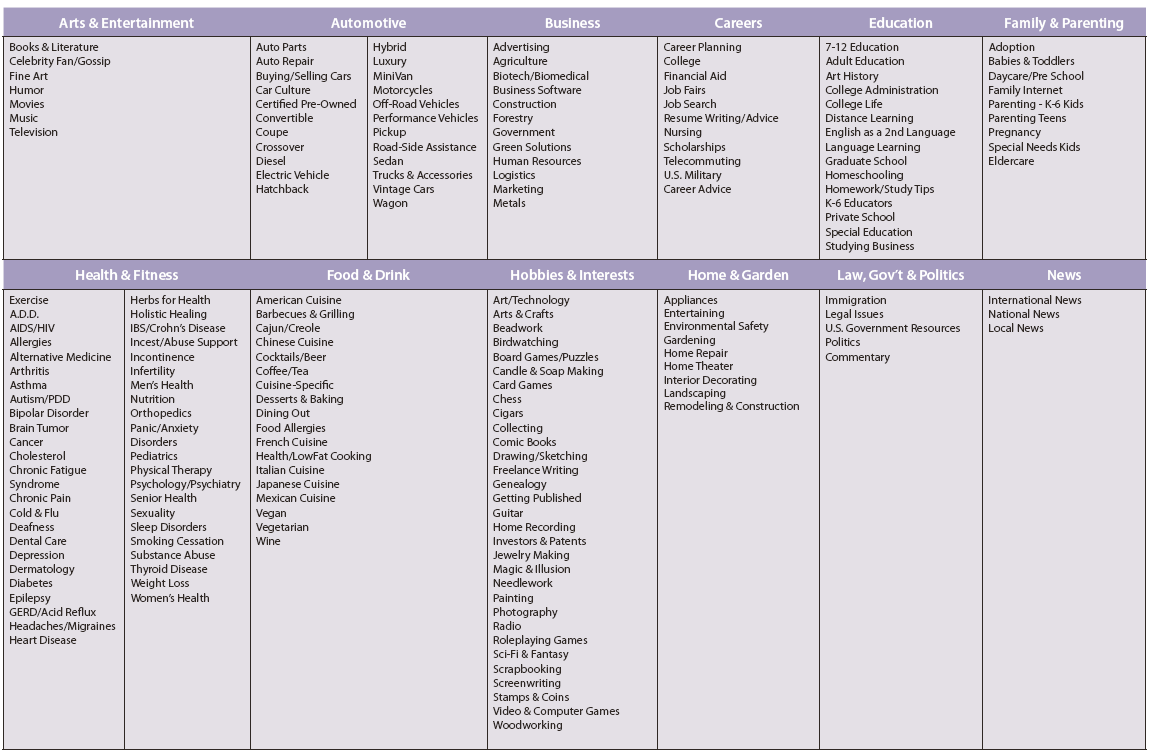
\includegraphics[width=1\textwidth]{IAB/Taxonomy-1.png}
\caption{Categories of the IAB Taxonomy}
\label{fig:IAB1}
\end{figure}
%\end{subfigure}
%\begin{subfigure}{\textwidth}
\begin{figure}[H]
\centering
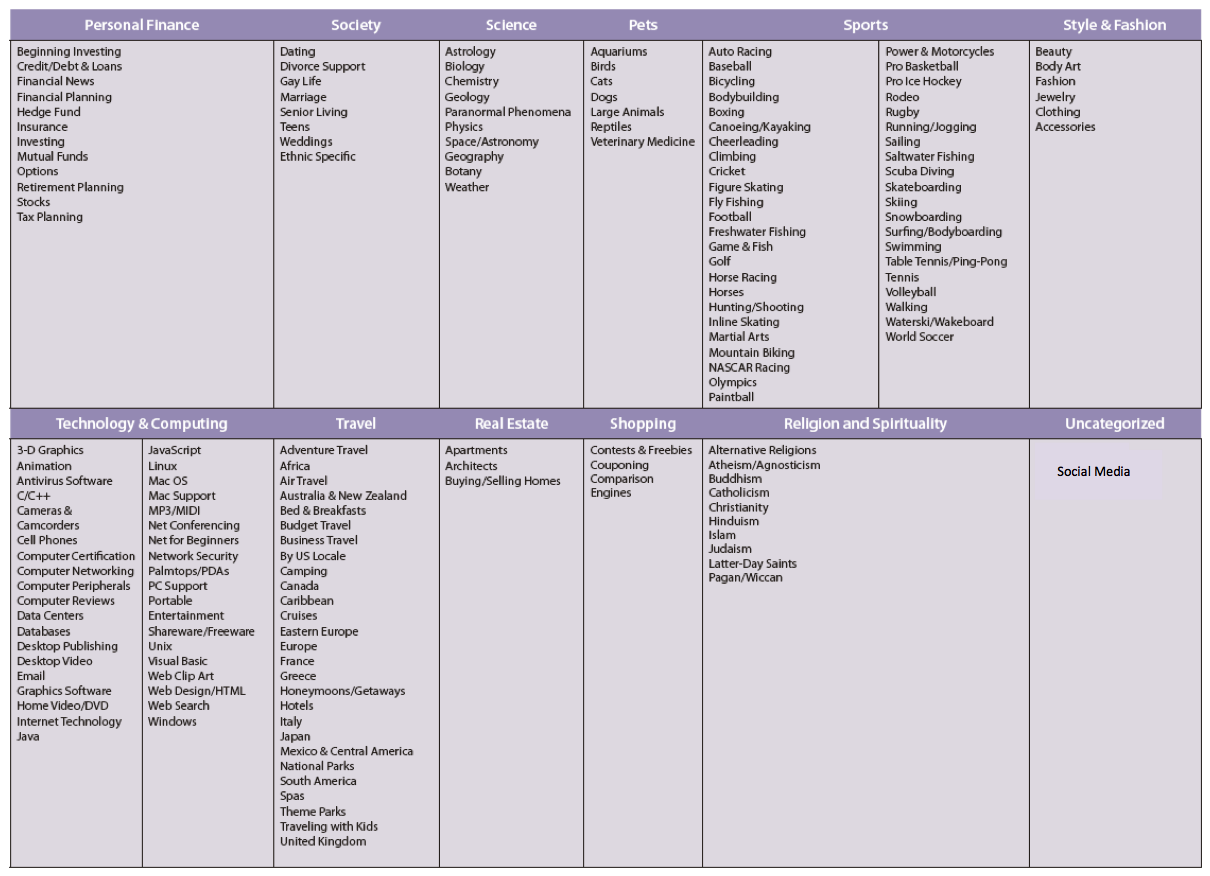
\includegraphics[width=1\textwidth]{IAB/Taxonomy-2.png}
%\end{subfigure}
\caption{Categories of the IAB Taxonomy}
\label{fig:IAB2}
%\label{fig:IAB-categories}
\end{figure}
%Figure \ref{fig:IAB-categories} 


%When categorizing a collection of texts, similar texts will be in the same cluster and therefore in the same category. This can be used to determine the content of the text. 

%The content analysis need a list of keyword to look for in texts. 

